\chapter{RDF}

Il \textbf{R}esource \textbf{D}escription \textbf{F}ramework è un linguaggio definito dal W3C per rappresentare informazioni semantiche sul web.

Le informazioni modellate con RDF sono strutturate secondo delle ontologie o dizionari: raccolte di classi e proprietà utili per descrivere un determinato contesto. Alcuni esempi di dizionari sono:

\begin{itemize}
	\item \textbf{Dublin Core} (dc):  un dizionario che contiene i termini per descrivere risorse multimediali e fisiche, come foto, video, libri, ecc.
	\item \textbf{Friend of a Friend} (foaf): un dizionario che contiene i termini per descrivere le reti sociali
	\item \textbf{Creative Commons Rights Expression Language} (ccREL): un dizionario per descrivere le informazioni riguardo la licenza con cui vengono pubblicati i contenuti multimediali che sono sotto licenze Creative Commons. Questi termini sono predisposti per essere inseriti all'interno di una pagina web utilizzando RDFa.
\end{itemize}

\noindent Queste informazioni vengono poi raggruppante e codificate in vario modo, un dei tanti è utilizzando \textbf{RDFa}, una serie di tag \textit{xhtml} che permetto di inserirle direttamente all'interno di una pagina web.

\section{Che cos'è RDF?}

RDF è un linguaggio di modellazione simile a quello ER o ai diagrammi delle classi, che si basa sulla definizione di \textbf{statement} (asserzioni) riguardanti delle \textbf{resources} nella forma \textit{soggetto-predicato-complemento}, con l'obiettivo che siano facilmente interpretabili sia da una persone che da un computer.

Ad esempio l'affermazione \textit{``il cielo è azzurro''} con RDF viene descritta come:

\begin{itemize}
	\item \textbf{Soggetto}: il cielo
	\item \textbf{Predicato} è di colore
	\item \textbf{Oggetto}: azzurro
\end{itemize}

Quando vengono descritte informazioni più complesse, può essere che un soggetto sia anche l'oggetto di altri statement, si parla quindi di:

\begin{itemize}
	\item \textbf{Risorse}: sono identificate da un URI e possono funzionare sia da soggetto che da oggetto. Possono anche essere definiti dei nodi anonimi con la sintassi \texttt{\_:\textit{identificatoreDelNodo}}.
	\item \textbf{Letterali}: un valore stringa primitivo che funziona solamente da oggetto. Utilizzando XSD è possibile specificare tipi diversi, come \texttt{xsd:integer} e \texttt{xsd:boolean}.
	\item \textbf{Proprietà}: il predicato della frase. Descrive un attributo o un aspetto di una risorsa e il valore della proprietà può essere sia un'altra risorsa che un letterale. Anche in questo caso è identificata da un URI. 
\end{itemize}

Un \textbf{URI} non è altro che un nome che viene dato ad una risorsa che si trova nel web e la scelta dell'URI da utilizzare viene lasciata all'utente.
Ad esempio per indicare la classe di vini Merlot è possibile utilizzare l'URI:

\begin{center}
	\texttt{http://www.w3.org/TR/2004/REC-owl-guide-20040210/wine\#Merlot}
\end{center}

Da notare che non è obbligatorio utilizzare un URL, ma se si vuole creare uno dizionario pubblico per descrivere una determinata categoria di informazioni può essere utile utilizzare un URL che porta alla descrizione del dizionario. Nell'esempio precedente l'URL porta alla definizione del dizionario \texttt{wine}.

Dato che gli URI possono essere molto lunghi e quindi possono rendere il documento di difficile comprensione è possibile utilizzare gli XML Qualified Name per creare un namespace.
Ad esempio l'URI precendete può essere abbreviato con 

\begin{center}
	\texttt{wine : http://www.w3.org/TR/2004/REC-owl-guide-20040210/wine}
\end{center}

\noindent così facendo ci si può riferire al Merlot utilizzando solamente \texttt{wine:Merlot}.

\subsection{Rappresentazione dei dati RDF}

Ci sono vari modi per rappresentare dati in formato RDF.
Come esempio per confrontare le varie sintassi viene utilizzata la frase:

\begin{center}
	\textit{C'è una persona identificata da \texttt{http://www.w3.org/People/EM/contact\#me}, che si chiama Eric Miller, che ha come indirizzo email e.miller123(at)example  e che ha il titolo di Dr.}
\end{center}

In questo caso si ha che gli oggetti sono: \textit{``Eric Miller''}, \textit{mailto:e.miller123(at)example} e \textit{``Dr.''}. L'unico soggetto è un URI e i vari predicati sono anch'essi identificati da un URI:

\begin{itemize}
	\item \textit{si chiama} : \texttt{http://www.w3.org/2000/10/swap/pim/contact\#fullName}
	\item \textit{ha come indirizzo email} : \texttt{http://www.w3.org/2000/10/swap/pim/contact\#mailbox}
	\item \textit{ha il titolo di} : \texttt{http://www.w3.org/2000/10/swap/pim/contact\#personalTitle}
\end{itemize}

Inoltre viene anche espresso il fatto che il soggetto ha un determinato tipo che è \textit{Persona}.

\subsubsection{N-Triple e Turtle}

Il formato più semplice per descrivere i dati in formato RDF è \textbf{N-Triple}, il quale consiste in un file di testo UTF-8 le cui linee o sono dei commenti che iniziano con \texttt{\#} oppure seguono la sintassi

\begin{center}
	\texttt{soggetto predicato complemento .}
\end{center}

La frase d'esempio viene rappresentata in N-Triple con:

\begin{lstlisting}
<http://www.w3.org/People/EM/contact#me> <http://www.w3.org/2000/10/swap/pim/contact#fullName> "Eric Miller" .
<http://www.w3.org/People/EM/contact#me> <http://www.w3.org/2000/10/swap/pim/contact#mailbox> <mailto:e.miller123(at)example> .
<http://www.w3.org/People/EM/contact#me> <http://www.w3.org/2000/10/swap/pim/contact#personalTitle> "Dr." .
<http://www.w3.org/People/EM/contact#me> <http://www.w3.org/1999/02/22-rdf-syntax-ns#type> <http://www.w3.org/2000/10/swap/pim/contact#Person> .
\end{lstlisting}

Una versione più avanzata di N-Triple è \textbf{Turtle} la quale permette sia di utilizzare dei prefissi per qualificare gli URI, sia di utilizzare altre notazioni avanzate.

Lo stesso esempio può essere riscritto con Turtle:

\begin{lstlisting}
@prefix eric:    <http://www.w3.org/People/EM/contact#> .
@prefix contact: <http://www.w3.org/2000/10/swap/pim/contact#> .
@prefix rdf:     <http://www.w3.org/1999/02/22-rdf-syntax-ns#> .

eric:me contact:fullName "Eric Miller" .
eric:me contact:mailbox <mailto:e.miller123(at)example> .
eric:me contact:personalTitle "Dr." .
eric:me rdf:type contact:Person .
\end{lstlisting}

\subsubsection{Rappresentazione grafica}

Le stesse informazioni possono essere rappresentate sotto forma grafica con un multi grafo orientato aciclico.

La notazione per standard per i grafi è:

\begin{itemize}
	\item \textbf{Risorse}: un ovale contenente l'URI.
	\item \textbf{Risorse anonime}: un cerchio vuoto.
	\item \textbf{Letterali}: un rettangolo contenente il valore.
	\item \textbf{Proprietà}: un arco avente l'URI della proprietà come etichetta.
\end{itemize}

\begin{figure}[htbp]
	\centering
	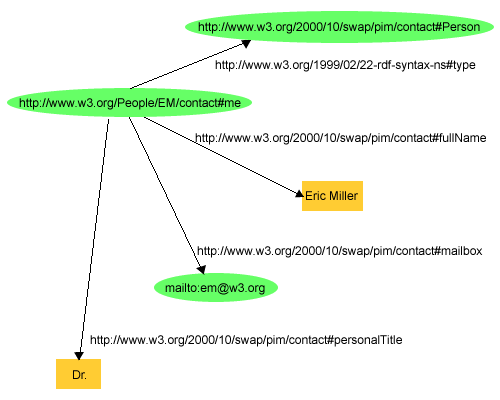
\includegraphics[width=.7\textwidth]{./images/miller_graph.png}
	\caption{Esempio di grafo RDF}
\end{figure}

\subsubsection{XML/RDF}

Esiste la possibilità di rappresentare i dati anche all'interno di un documento XML, anche se questo formato viene scarsamente utilizzato perché molto verboso e non permette di rappresentare tutti i tipi di grafi.

\begin{lstlisting}
<?xml version="1.0" encoding="utf-8"?>
<rdf:RDF xmlns:contact="http://www.w3.org/2000/10/swap/pim/contact#" xmlns:eric="http://www.w3.org/People/EM/contact#" xmlns:rdf="http://www.w3.org/1999/02/22-rdf-syntax-ns#">
	<rdf:Description rdf:about="http://www.w3.org/People/EM/contact#me">
		<contact:fullName>Eric Miller</contact:fullName>
	</rdf:Description>
	<rdf:Description rdf:about="http://www.w3.org/People/EM/contact#me">
		<contact:mailbox rdf:resource="mailto:e.miller123(at)example"/>
	</rdf:Description>
	<rdf:Description rdf:about="http://www.w3.org/People/EM/contact#me">
		<contact:personalTitle>Dr.</contact:personalTitle>
	</rdf:Description>
	<rdf:Description rdf:about="http://www.w3.org/People/EM/contact#me">
		<rdf:type rdf:resource="http://www.w3.org/2000/10/swap/pim/contact#Person"/>
	</rdf:Description>
</rdf:RDF>
\end{lstlisting}

\section{Containers e Collections RDF}

I \textbf{container} vengono utilizzati per rappresentare dei gruppi di cose, come la lista degli autori di un libro.

Ci sono 3 tipi di container:

\begin{itemize}
	\item \texttt{rdf:Bag}: rappresenta una lista non ordinata di oggetti
	\item \texttt{rdf:Seq}: rappresenta una lista ordinata di oggetti.
	\item \texttt{rdf:Alt}: rappresenta una lista di valori alternativi, dei i quali solo un può essere selezionato.
\end{itemize}
\FloatBarrier
\begin{lstlisting}[caption=Esempio di Bag con XML/RDF]
<?xml version="1.0"?>
<rdf:RDF
xmlns:rdf="http://www.w3.org/1999/02/22-rdf-syntax-ns#" 
xmlns:cd="http://www.recshop.fake/cd#"> 
	<rdf:Description rdf:about="http://www.recshop.fake/cd/Beatles">
		<cd:artist>
			<rdf:Bag>
				<rdf:li>John</rdf:li>
				<rdf:li>Paul</rdf:li>
				<rdf:li>George</rdf:li>
				<rdf:li>Ringo</rdf:li>
				</rdf:Bag>
				</cd:artist>
		</rdf:Description>
</rdf:RDF>
\end{lstlisting}

\begin{lstlisting}[caption=Bag con N-Triple]
exstaff:Sue exterms:publication _:z .
_:z rdf:type rdf:Bag .
_:z rdf:_1 ex:AnthologyOfTime .
_:z rdf:_2 ex:ZoologicalReasoning .
_:z rdf:_3 ex:GravitationalReflections . 
\end{lstlisting}

Nella rappresentazione grafica vengono utilizzate delle proprietà \textit{anonime?} con un URI che avanza progressivamente.
\FloatBarrier
\begin{figure}[htbp]
	\centering
	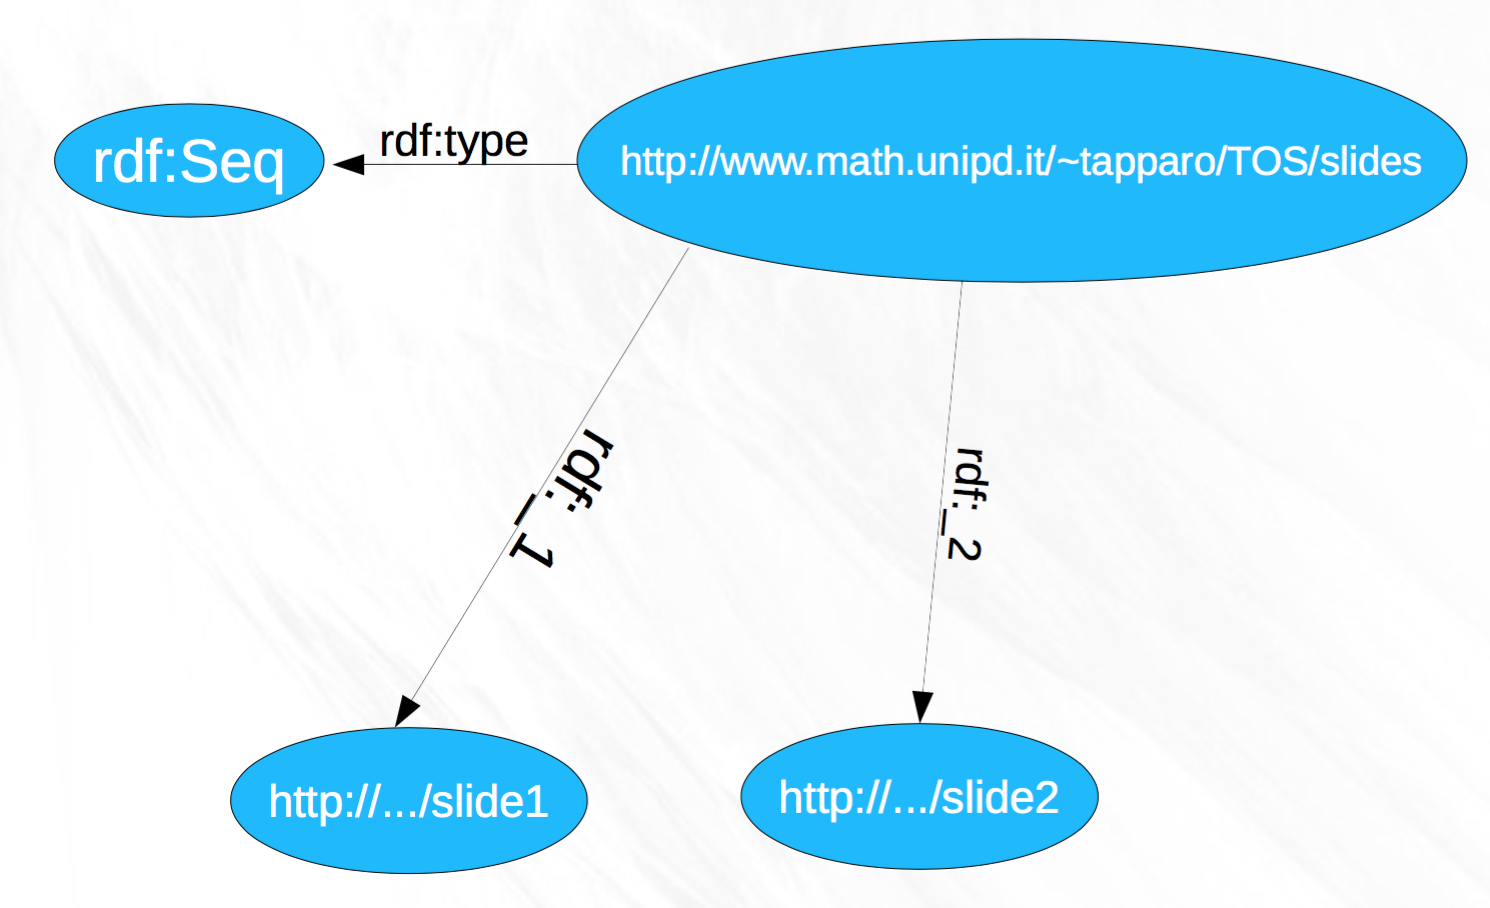
\includegraphics[width=.4\textwidth]{./images/seq_graph.png}
	\caption{Grafo RDF con \texttt{rdf:Seq}}
\end{figure}

I container però non sono bloccabili, ovvero possono essere aggiunti nuovi elementi.
Se invece si vuole limitare il numero di elementi che possono essere presenti all'interno del contenitore è necessario utilizzare una \textbf{Collection}.

Le collezioni RDF sono rappresentate come una lista singolarmente linkata e viene definita utilizzando le proprietà \texttt{rdf:first}, \texttt{rdf:rest} e \texttt{rdf:nil}.

\begin{figure}[htbp]
	\centering
	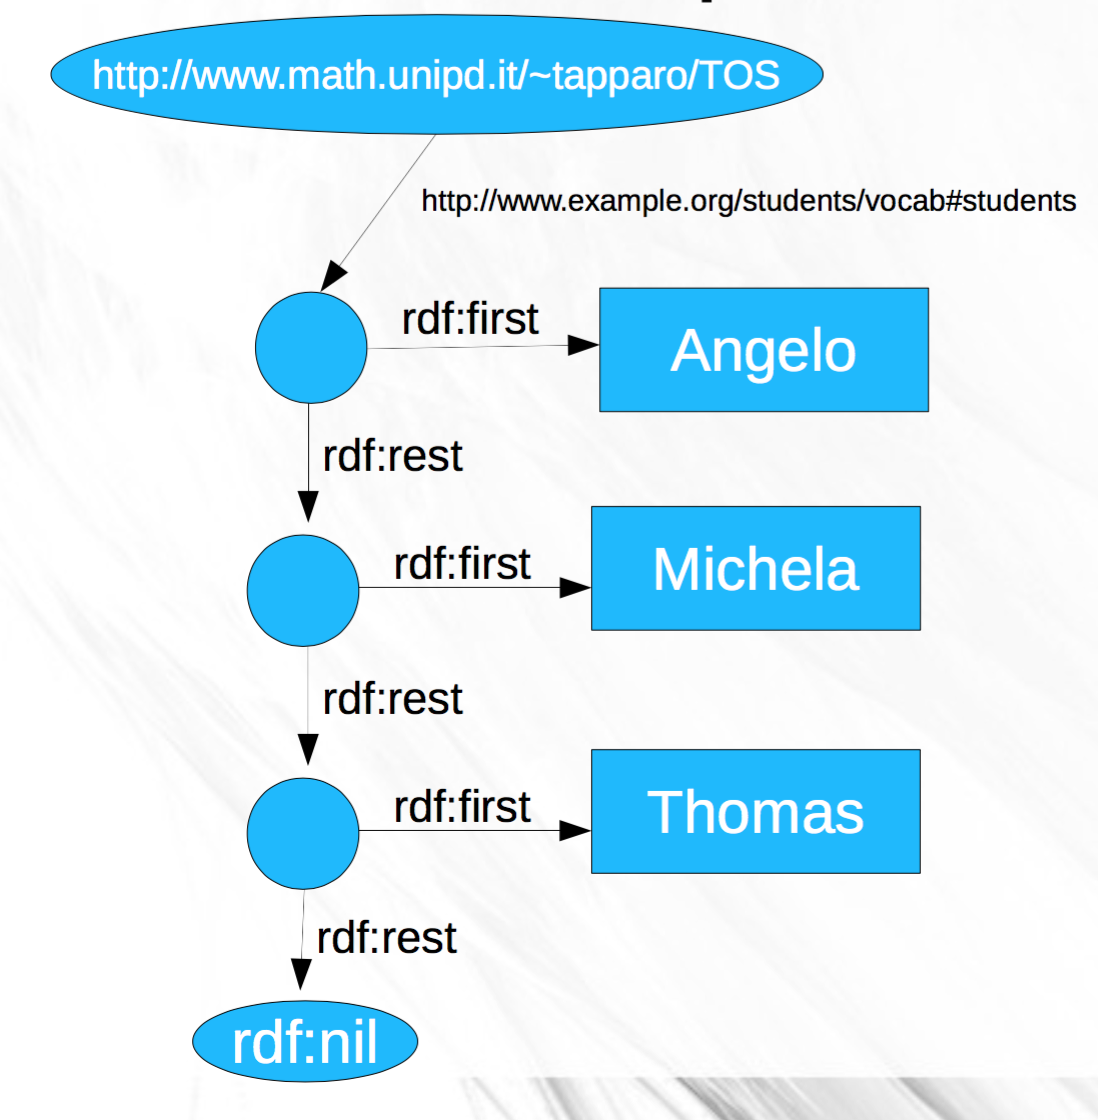
\includegraphics[width=.4\textwidth]{./images/list_graph.png}
	\caption{Grafo RDF con una collezione}
\end{figure}

La definizione di una lista con N-Triple viene fatta definendo i vari nodi:

\begin{lstlisting}[caption=Definzione di una lista con N-Triple]
http://www.math.unipd.it/~tapparo/TOS http://www.example.org/students/vocab#students _:sl
_:sl rdf:first "Angelo"
_:sl rdf:next _:sl2
_:sl2 rdf:first "Michela"
_:sl2 rdf:next _:sl3
_:sl3 rdf:first "Thomas"
_:sl3 rdf:next rdf:nil
\end{lstlisting} 

\section{Reification}

RDF permette di descrivere degli statement RDF utilizzando RDF, mediante un vocabolario built-in.

Questo vocabolario permette contiene la classe \texttt{rdf:Statement} che specifica il tipo del nodo e i predicati: \texttt{rdf:subject}, \texttt{rdf:predicate} e \texttt{rdf:object}.

Ad esempio mediante la reificazione è possibile esprimere:

\begin{center}
	\textit{Angelo ha detto che il corso di TOS è tenuto da Francesco Tapparo.}
\end{center}

\begin{lstlisting}[caption=Reification con N-Triple, language=RDFA]
# Frase detta da angelo
_:frase rdf:type rdf:Statement
_:frase rdf:subject <http://www.math.unipd.it/~tapparo/TOS/>
_:frase rdf:predicate dc:creator
_:frase rdf:object "Francesco Tapparo"

# Specifico che la farse è detta da Angelo
_:frase dc:creator _:ang
_:ang foaf:name "Angelo"
_:ang rdf:type foaf:Person
\end{lstlisting}

\begin{figure}[htbp]
	\centering
	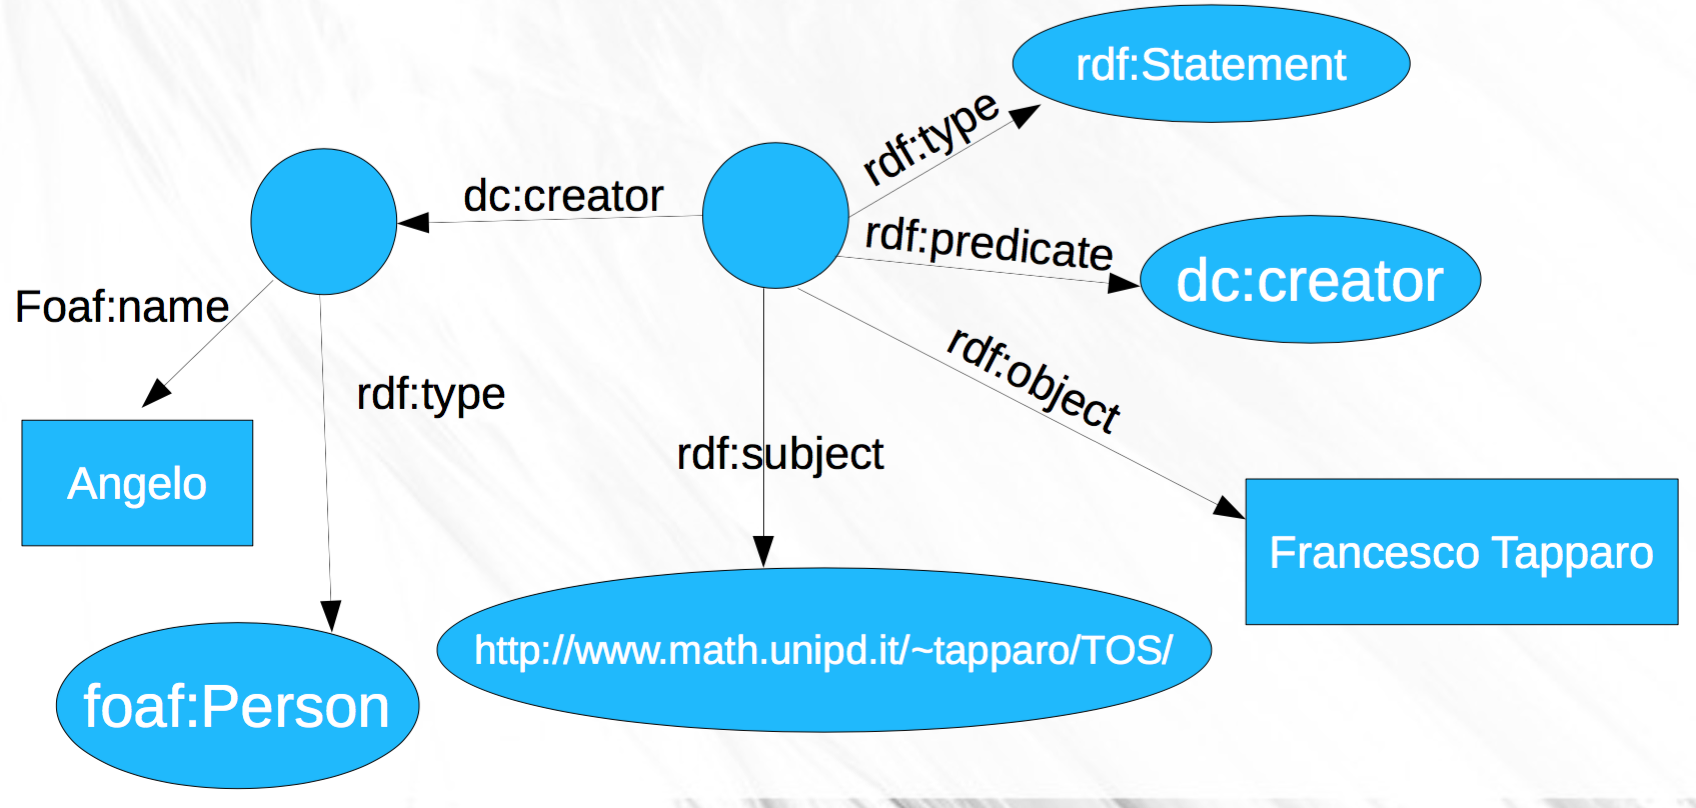
\includegraphics[width=.5\textwidth]{./images/reif_graph.png}
	\caption{Grafo RDF per: \textit{Angelo ha detto che il corso di TOS è tenuto da Francesco Tapparo.}}
\end{figure}

\section{RDFa}

RDFa è uno standard W3C che aggiunge una serie di attributi all'HTML e XHTML che permettono di inserire all'interno dei documenti i metadati RDF.

Così facendo non è più necessario mantenere un file separato con le informazioni RDF relative alla pagina web, in quanto questo può essere estratto utilizzando un distiller come \texttt{pyRdfs}\footnote{\url{https://www.w3.org/2012/pyRdfa/}}.

\subsection{Prefissi iniziali - CURIE}

Anche con RDFa è possibile utilizzare una notazione di prefissi (\textbf{CURIE}) che permette di accorciare gli URI e facilitare la comprensione all'essere umano.

Per utilizzare i prefissi basta aggiungere ad un tag la definizione del namespace, utilizzando l'attributo \texttt{xmlns}.
Una volta dichiarato il namespace, è possibile utilizzare il prefisso su tutti i tag discendenti.

\begin{lstlisting}[language=RDFA]
<html xmlns="..." xmlns:dc="http://purl.org/dc/terms/" > 
...
<!-- permette di utilizzare il prefisso dc -->
<span property="dc:description">Valore</span>

<!-- al posto di -->
<!-- property="http://purl.org/dc/terms/:description" -->
...
</html>
\end{lstlisting}

\noindent Tuttavia questo sistema utilizza i namespace XML.

Un'alternativa è quella di definire un vocabolario di default utilizzando \textbf{\texttt{vocab}} che funziona in modo simile, solo che non è possibile specificare il prefisso.
Se si vogliono utilizzare altri vocabolari è necessario specificare l'URI completo.

\begin{lstlisting}[caption=Utilizzo di vocab, language=RDFA]
...
<body vocab="http://purl.org/dc/terms/">
<h2 property="title">The Trouble with Bob</h2>
<p>Date: <span property="created">2011-09-10</span></p> </body>
...
\end{lstlisting}

\noindent Esiste anche un'altra alternativa data dall'attributo \textbf{\texttt{prefix}} che funziona in modo simile alla definizione del namespace e che può essere utilizzato assieme a \texttt{vocab}.

\begin{lstlisting}[caption=Utilizzo di prefix, language=RDFA]
<body prefix="p1: http://www.p1.org/ p2: http://222.p2.org"> 
	<span property="p1:property">proprietà 1</span>
	<span property="p2:property">proprietà 2</span>
</body>
\end{lstlisting}

\subsection{Individuare i predicati}

Il predicato di una tripla viene specificato attraverso gli attributi \texttt{property} o \texttt{rel}.
Questi attributi possono essere aggiunti a qualunque tag del documento e possono assumere come valore un URI, un CURIE o una lista di CURIES sperati da uno spazio.

\begin{lstlisting}[caption=Utilizzo di property, language=RDFA]
<div xmlns:dc="..." about="http://aBook.org">
	<span property="dc:title">aTitle</span>
	<span property="dc:creator">aCreator</span>
</div>

<!--
	Equivale a:
	http://aBook.org dc:title "aTitle" .
	http://aBook.org dc:creator "aCreator" .
-->
\end{lstlisting}

La differenza tra i due modi per specificare il predicato riguarda il come viene scelto l'oggetto.

\subsection{Individuare gli oggetti}

Come anticipato, il modo di identificare gli oggetti cambia in base a come viene specificato il predicato.

Se viene usato \texttt{property}, l'oggetto viene scelto utilizzando una delle seguenti regole. Se non è possibile identificarlo con la prima, si passa alla successiva e così via.

\begin{enumerate}
	\item Il valore dell'attributo \texttt{content}. Es: \texttt{<span about="..." property="foaf:name" content="Giacomo"/>}.
	\item Il valore dell'attributo \texttt{resource} e se il tag \texttt{datatype} non è presente.
	\item Il valore dell'attributo \texttt{href} e se il tag \texttt{datatype} non è presente.
	\item Il valore dell'attributo \texttt{src} e se il tag \texttt{datatype} non è presente.
	\item Il contenuto effettivo del tag.
\end{enumerate}

Se invece il predicato viene specificato con \texttt{rel} le regole sono le stesse, solo che non viene preso in considerazione il primo punto e nel punto 5, al posto del contenuto del tag viene preso in considerazione l'URI del tag, ovvero viene creato un nodo bianco

\begin{lstlisting}[language=RDFA, caption=La pagina web creata da Alice]
<html xmlns:dc="http://purl.org/dc/elements/1.1/"> 
	<head>
		<meta property="dc:title" content="Alice's web page" />
		<meta property="dc:creator" content="Alice" />
	</head>
	<body>...</body>
</html>
\end{lstlisting}

\`E inoltre possibile specificare il tipo degli oggetti utilizzando il tag \texttt{datatype} e le definizioni xsd, ad esempio:

\begin{lstlisting}[language=RDFA]
	<span about="..." property="..." datatype="xsd:integer">10</span>
\end{lstlisting}

Da notare che il valore degli attributi \texttt{resource}, \texttt{href} e \texttt{src} deve essere un URI.

\subsection{Individuare i soggetti}

Per identificare il soggetto dei vari statement RDF viene utilizzato o il tag HTML che ha tra i suoi attributi in predicato, oppure il suo tag genitore immediatamente superiore che lo contiene.

Per specificare il soggetto iniziale è possibile utilizzare il tag \texttt{<base href="..."/>} il quale viene utilizzato dai vari parser e browser per risolvere i link relativi. Tipicamente viene quindi settato al l'URL della pagina web.
Può esserci al massimo uno di questi tag e deve essere inserito all'interno del \texttt{<head>}.

Altrimenti è possibile specificare il soggetto utilizzando l'attributo \texttt{about}.

\begin{lstlisting}[language=RDFA, caption=Utilizzo di about]
<div about="/barbecue">
	<h2 property="dc:title">Joe's Barbecue</h2>
</div>
<!--
	Equivale a:
	 "urlDellaPagina"/barbecue dc:title "Joe's Barbecue" .
-->
\end{lstlisting}

Utilizzando l'attributo \texttt{about} è possibile definire in modo esplicito dei nodi anonimi:

\begin{lstlisting}[language=RDFA, caption=Utilizzo di about]
<link about="[_:n1]" rel="foaf:mbox" href="mailto:john@ex.org" />
<link about="[_:n2]" rel="foaf:mbox" href="mailto:sue@ex.org" />
<link about="[_:n1]" rel="foaf:knows" href="[_:n2]" />
</div>
<!--
	Equivale a:
	_:n1 foaf:mbox <mailto:john@ex.org> .
	_:n2 foaf:mbox <mailto:sue@ex.org> .
	_:n1 foaf:knows _:n2 .
-->
\end{lstlisting}

Un altro modo per impostare il soggetto è dato dall'attributo \texttt{typeof} che definisce la tipologia della risorsa soggetto e determina il soggetto per tutte le triple RDF definite nel blocco di codice incluso nel tag al quale è applicato. Il soggetto utilizzato è un nuovo nodo anonimo.

\begin{lstlisting}[language=RDFA, caption=Utilizzo di typeof]
<div typeof="foaf:Person">
	<p property="foaf:name">Alice</p> 
	<p>
		Email: <a rel="foaf:mbox" href="mailto:alice@example.com">alice@example.com</a>
	</p>
	<p>
		Phone: <a rel="foaf:phone" href="tel:0444123456">0444123456</a>
	</p>
</div>
<!--
	Equivale a:
	_:n1 rdf:type foaf:Person .
	_:n1 foaf:name "Alice" .
	_:n1 foaf:mbox <mailto:alice@example.com> .
	_:n1 foaf:phone <tel:0444123456> .
-->
\end{lstlisting}

\subsection{Chaining}

Per definire i predicati è possibile utilizzare anche l'attributo \texttt{rel}, il quale abilita il chaining, ovvero quel meccanismo che permette di collegare l'oggetto di uno statement al soggetto di un altro statement.

Si ha quindi che con il chaining l'oggetto dello statement esterno diventa il soggetto di quello interno, oppere il soggetto della proposizione interna diventa l'oggetto di quella esterna.

\begin{lstlisting}[language=RDFA, caption=Esempi di chaining]
<a about="http://www.debian.org" rel="dc:creator" href="http://www.ian.org">
	<span property="foaf:name">Ian Murdock</span>
</a>
<!--
	<http://www.debian.org> dc:creator <http://www.ian.org> .
	<http://www.ian.org> foaf:name "Ian Murdoc"
-->
<div about="#me" rel="foaf:knows">
	<div 
		about="http://www.w3.org/People/Ivan/#me"
		property="foaf:name"
		content="Ivan Herman" />
</div>
<!--
	<#me> foaf:knows <http://www.w3.org/People/Ivan/#me> .
	<http://www.w3.org/People/Ivan/#me> foaf:name "Ivan Herman" .
-->
\end{lstlisting}

\begin{lstlisting}[language=RDFA, caption=Io conosco pino che conosce gino che ha una determinata foto]
<div about="#me" rel="foaf:knows">
	<div about="http://www.pino.org/#me"
		rel="foaf:knows"
		href="http://www.gino.org">
		<img rel="foaf:depiction" src="http://www.gino.org/pic.jpg" />
	</div>
</div>
<!-- 
	<#me> foaf:knows <http://www.pino.org/#me> .
	<http://www.pino.org/#me> foaf:knows <http://www.gino.org> .
	<http://www.gino.org> foaf:depiction <http://www.gino.org/pic.jpg> .
-->
\end{lstlisting}

Se non viene specificato né un oggetto per la proposizione esterna, né un soggetto per quella interna, il collegamento tra le due è fornito da un nodo anonimo creato automaticamente (\textbf{chaining con intermediario anonimo}).

\begin{lstlisting}[language=RDFA, caption=Utilizzo del chaining anonimo]
<div about="#me" rel="foaf:knows">
	<div property="foaf:name">Francesco Tapparo</div>
</div>
<!--
	<#me> foaf:knows _:n1 .
	_:n1 foaf:name "Francesco Tapparo" .
-->
\end{lstlisting}

\subsubsection{Esercizi dalle slide}

Utilizzando il chaining è possibile utilizzare le così dette \textbf{triple incomplete}:

\begin{center}
\textit{``Albert Einstein è vissuto in germania e svizzera''}
\end{center}

\begin{lstlisting}[language=RDFA]]
<div about="http://dbpedia.org/resource/Albert_Einstein">	
	<div rel="dbp-owl:residence" resource="http://dbpedia.org/resource/German_Empire">
	</div>
	<div rel="dbp-owl:residence" resource="http://dbpedia.org/resource/Switzerland">
	</div>
</div>
<!--
	<http://dbpedia.org/resource/Albert_Einstein>  dbp-owl:residence <http://dbpedia.org/resource/German_Empire> .
	<http://dbpedia.org/resource/Albert_Einstein>  dbp-owl:residence <http://dbpedia.org/resource/Switzerland> .
-->
\end{lstlisting}

\begin{center}
	\textit{``La foto ... rappresenta Albert Einstein''}
\end{center}

\begin{lstlisting}[language=RDFA]
<div about="http://dbpedia.org/resource/Albert_Einstein" rel="foaf:depiction">
	<img src="http://dbpedia.org/einstein.jpg" />
</div>
<!-- 
	<http://dbpedia.org/resource/Albert_Einstein> foaf:depiction <http://dbpedia.org/einstein.jpg> .
	In questo caso è src che identifica l'oggetto perché il predicato è definito con rel
-->
\end{lstlisting}

\begin{center}
	\textit{``Specificare sul proprio sito un insieme di persone che si conoscono insieme ai rispettivi siti web e indirizzi email''}
\end{center}

\begin{lstlisting}[language=RDFA]
<ul about="#me">
	<li rel="foaf:knows" href="http://www.ftapparo.org/#me">
		<span property="foaf:name">Francesco<span> (<a rel="foaf:mbox" href="mailto:tapparo@math.unipd.it
">email</a>)
	</li>
</ul>
<!-- 
	<#me> foaf:knows <http://www.ftapparo.org/#me> .
	<http://www.ftapparo.org/#me> foaf:name "Francesco" .
	<http://www.ftapparo.org/#me> foaf:mbox <"mailto:tapparo@math.unipd.it> .
-->
\end{lstlisting}

\begin{center}
	\textit{``Specificare che il proprio post è sotto licenza CC-BY-NC ma che un'immagine contenuta è sotto licenza CC-BY''}
\end{center}

\begin{lstlisting}[language=RDFA]
<a rel="license" href="http://www.creativecommons.org/rel/cc-by-nc">CC-BY-NC</a>
<img about="/img.jpg" src="/img.jpg" rel="license" href="http://www.creativecommons.org/rel/cc-by" />
<!-- 
	<http://www.ex.org/> license <http://www.creativecommons.org/rel/cc-by-nc> .
	<http://www.ex.org/img.jpg) license <http://www.creativecommons.org/rel/cc-by> .
-->
\end{lstlisting}

\begin{center}
	\textit{``Specificare sul proprio sito web i contatti''}
\end{center}

\begin{lstlisting}[language=RDFA]
<span rel="dc:creator" resource="[_:me]">
	<b property="foaf:name">Francesco Tapparo</b> (<em rel="foaf:mbox" href="mailto:myemail@gmail.com">
contattami</em>) </span>
<!-- 
	</> dc:creator _:me .
	_:me foaf:name "Francesco Tapparo" .
	_:me foaf:mbox <mailto:myemail@gmail.com> .
-->
\end{lstlisting}

\section{RDF Schema}

\`E un linguaggio per definire dei vocabolari per RDF.

Alla base di RDFS c'è \texttt{rdfs:Resource}, tutti gli elementi utilizzati da RDFS sono risorse. Ci sono poi le classi \texttt{rdfs:Class} che definiscono un particolare tipo di risorsa e che possono essere assegnate utilizzando la proprietà \texttt{rdf:type}.

\begin{lstlisting}[language=RDFA]
	# Definisco la classe Person
	ex:Person rdf:type rdfs:Class .
	# Speficifo la classe di una risorsa
	ex:Giacomo rdf:type ex:Person .
\end{lstlisting} 

Le proprietà sono invece definite utilizzando la classe \texttt{rdfs:Property} e vengono utilizzate per definire una relazione che c'è tra una risorsa soggetto e una risorsa oggetto.

La definizione di una proprietà viene fatta in modo analogo alla definizione di una classe:

\begin{lstlisting}
	ex:nome rdf:type rdfs:Property .
	ex:Giacomo ex:nome "Giacomo" .
\end{lstlisting}

Una proprietà che è già presente all'interno di RDFS è \texttt{rdfs:subClassOf} che permette di definire delle gerarchie di classi secondo la regola:

\begin{center}
\textit{``A è sotto classe di B se ogni istanza di A è anche istanza di B''}
\end{center}

Quindi per dire che la classe \texttt{foaf:Agent} deriva da \texttt{foaf:Person} la sintassi è

\begin{lstlisting}
	foaf:Person rdfs:subClassOf foaf:Agent .
\end{lstlisting} 

Le classi RDFS non sono tipate e quindi qualsiasi proprietà può essere associata ad una istanza di una determinata classe.
Le proprietà invece sono tipate, ovvero possono essere applicate solo a determinate classi di risorse. Per specificare ciò è necessario utilizzare \texttt{rdfs:domain} per impostare il tipo del soggetto e \texttt{rdfs:range} per il tipo dell'oggetto.

\begin{lstlisting}
	:Book rdf:type rdfs:Class .
	:bookTitle rdf:type rdf:Property .
	:bookTitle rdfs:domain :Book .
	:bookTitle rdfs:range rdfs:Literal .
	:MyBook rdf:type :Book .
	:MyBook :bookTitle "My Book" .
\end{lstlisting}

In RDFS è possibile modellare anche le sotto proprietà, ovvero specificare che tutte le risorse che sono collegate da una proprietà sono anche collegate da un'altra.

\begin{lstlisting}
	:involves rdfs:subPropertyOf :isTautghtBy
	<!-- Se un corso è tenuto da una risorsa vale anche il fatto che il corso coinvolge quella risorsa-->
\end{lstlisting}

Le proprietà \texttt{rdfs:subPropertyOf} e \texttt{rdfs:subClassOf} sono anche transitive.

\subsection{Altri predicati di utilità}

\begin{itemize}
	\item \texttt{rdfs:comment}: viene utilizzato per fornire una descrizione testuale di una risorsa.
	\item \texttt{rdfs:label}: viene utilizzato per fornire un nome comprensibile ad una persona per una determinata risorsa.
	\item \texttt{rdfs:seeAlso}: viene utilizzato per indicare un'altra risorsa che può fornire ulteriori informazioni riguardo il soggetto.
	\item \texttt{rdfs:isDefinedBy}: viene utilizzato per specificare una risorsa che definisce il soggetto. Viene utilizzata per indicare il vocabolario RDF contenente la definizione della risorsa.
\end{itemize}

\subsection{Esempio di RDFS}

\begin{lstlisting}
	:Course rdf:type rdfs:Class .
	:Lecturer rdf:type rdfs:Class .
	:AccademicStaffMember rdf:type rdfs:Class .
	:StaffMember rdf:type rdfs:Class .
	
	:StaffMember rdfs:subClassOf :AccademicStaffMember .
	:AccademicStaffMember rdfs:subClassOf :Lecturer .
	
	:isTaughtBy rdf:type rdfs:Property .
	:involves rdf:type rdfs:Property .
	
	:involves rdfs:subPropertyOf :isTaughtBy .
	:involves rdfs:domain :Course .
	:involves rdfs:range :Lecturer
	
	:Lecturer rdfs:comment "La classe che rappresenta gli insegnati"
\end{lstlisting}

\subsection{Dublin Core}

Vocabolario che contiene le proprietà relative al contenuto di un opera, alcune di queste sono \texttt{dc:title}, \texttt{dc:subject}, \texttt{dc:description} e \texttt{dc:source}.

Sono inoltre contenute delle altre proprietà che esprimono in modo più dettagliato le informazioni sulla proprietà intellettuale come: \texttt{dc:creator}, \texttt{dc:contributor}, \texttt{dc:publisher} e \texttt{dc:rights}. Quest'ultima viene utilizzata per fornire un link alla licenza.

Un'altro predicato importante è \texttt{dc:mitype} che specifica la tipologia del documento. I valori più utilizzati sono \texttt{dcmitype:Text}, \texttt{dcmitype:Sound}, \texttt{dcmitype:StillImage} e \texttt{dcmitype:MovingImage}.

\subsection{ccREL}

Vocabolario che contiene i termini per la definizione delle licenze.

Le proprietà definite nel vocabolario si dividono in \textbf{work properties} e \textbf{license properties}.

Quelle relative all'opera sono:

\begin{itemize}
	\item \texttt{cc:license}: utilizzata per specificare l'URI della licenza, equivale ad utilizzare \texttt{xhtml:license} ed è una sotto proprietà di \texttt{dc:license}.
	\item \texttt{cc:attributionName}: nome da utilizzare per dare credito all'autore dell'opera.
	\item \texttt{cc:attributionUrl}: URL da utilizzare per dare credito all'autore dell'opera.
	\item \texttt{cc:morePermission}: URI di una risorsa che descrive ulteriori permessi oppure una licenza alternativa.
\end{itemize}

Viene inoltre consigliata l'aggiunta dei predicati \texttt{dc:title} e \texttt{dc:mitype}.

Le \textbf{license properties} descrivono invece le condizioni della licenza, quello che viene permesso, i requisiti per utilizzare l'opera e cosa non è possibile fare.


\subsubsection{Esempio}

\begin{center}
	\textit{``Specificare che il brano pippo.mp3 dal titolo 'Pippi Oh' scritto da Pippo è rilasciato sotto licenza CC-BY-NC-ND ma è possibile acquistare ulteriori diritti visitando \texttt{http://www.depippis.org/buy.php}''}
\end{center}

\begin{lstlisting}[language=RDFA]
<div about="/pippo.mp3">
	<span rel="dc:mitype" resource="dcmitype:Sound" />
	<span rel="dc:title">Pippi Oh</span>
	<span rel="cc:license" href="http://www.creativecommons.org/rel/cc-by-nc-nd">CC-BY-NC-ND</span>
	<a rel="cc:morePermission" href="http://www.depippis.org/buy.php">Buy more </a>
</div>
<!--
	</pippo.mp3> dc:mitype dcmitype:Sound .
	</pippo.mp3> dc:title "Pippi Oh" .
	</pippo.mp3> cc:license <http://www.creativecommons.org/rel/cc-by-nc-nd> .
	</pippo.mp3> cc:morePermission <http://www.depippis.org/buy.php> .
-->
\end{lstlisting}
